\documentclass[10pt,a4paper]{article}
\usepackage[utf8]{inputenc}
\usepackage{amsmath}
\usepackage{amsfonts}
\usepackage{amssymb}
\usepackage{graphicx}
\usepackage{enumerate}
\begin{document}

\section{Set Theory}

To demystify mathematics consider
\begin{enumerate}[(i)]
\item What is a theorem?
\item What is a proof?
\end{enumerate}
What if we don't know the answer?

To begin we need
\begin{enumerate}[(a)]
\item an example(s)
\item a nearly related concept
\end{enumerate}


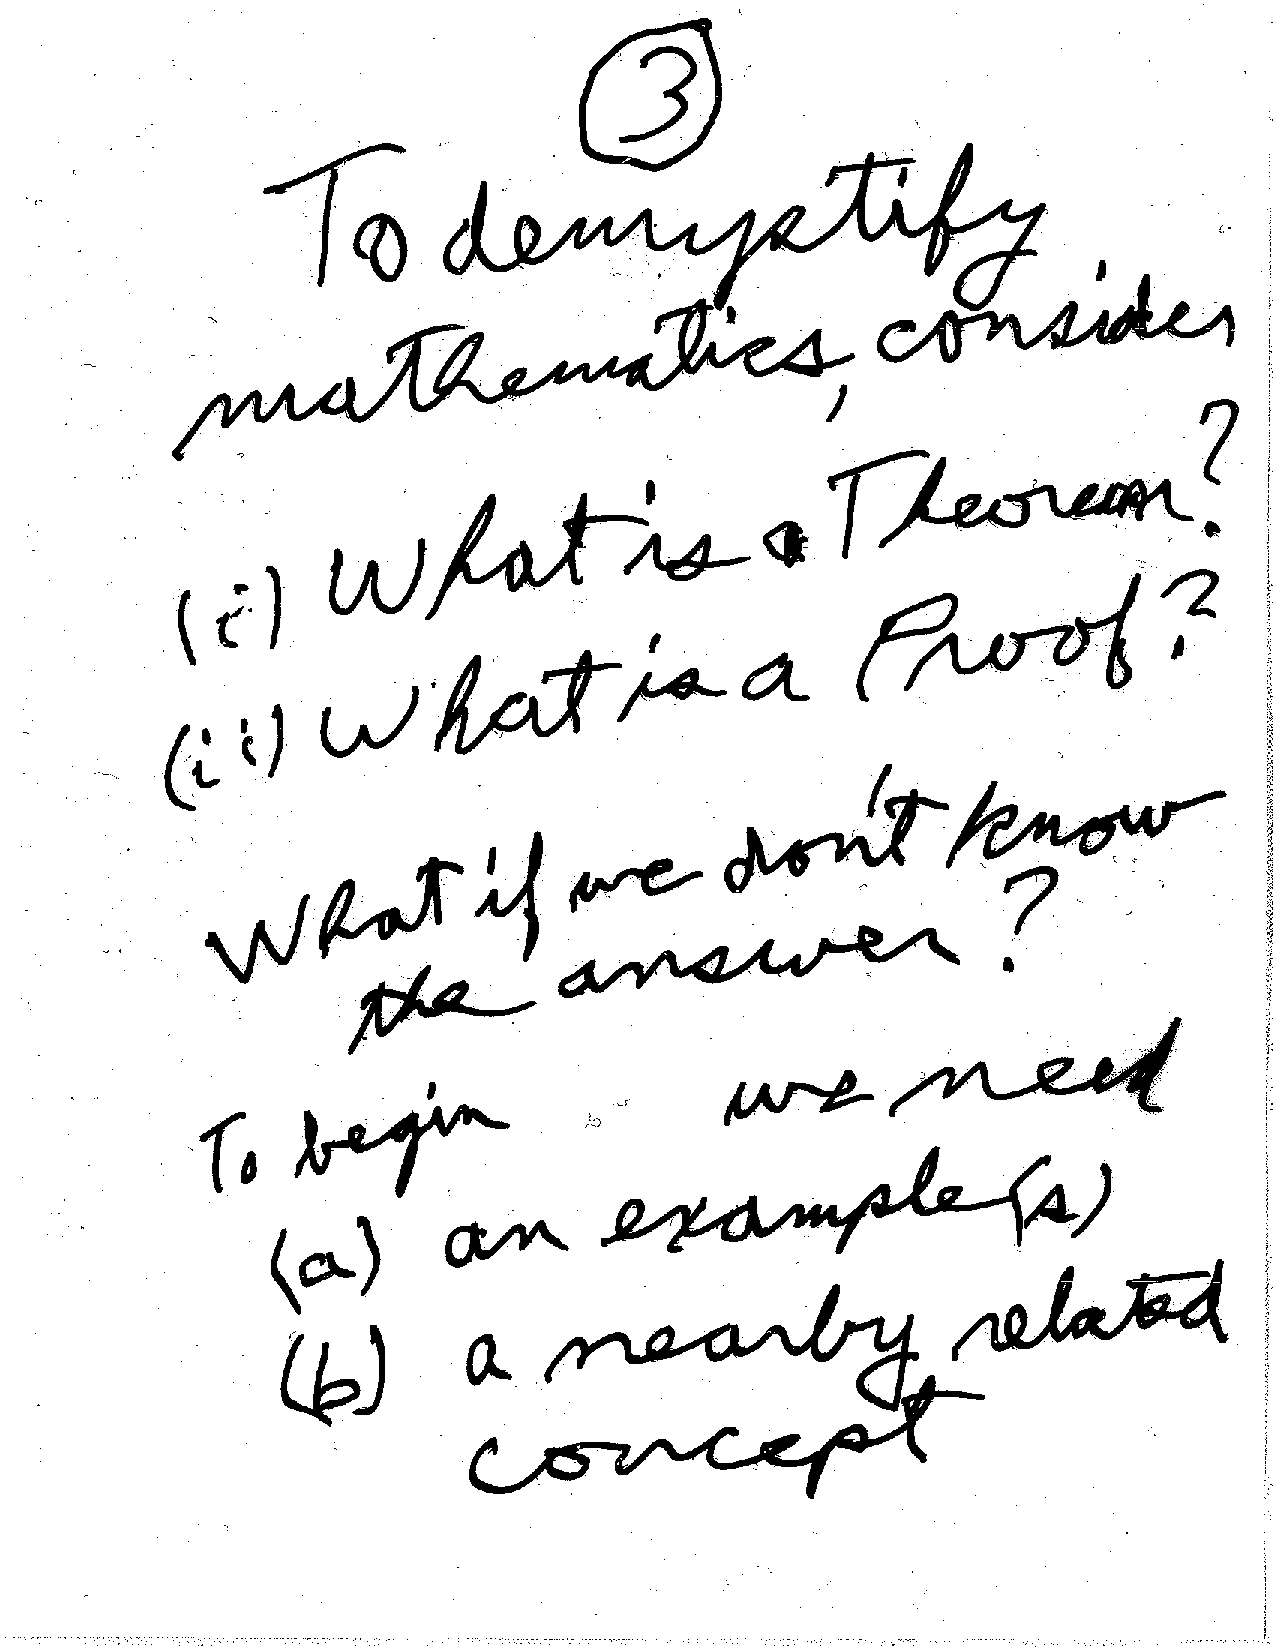
\includegraphics[scale=.5]{Pages/ST_3}

\newpage

Related Concept: Greek Syllogism

\underline{example:}
\begin{enumerate}
\item All men are mortal.
\item Socrates is a man.
\item Therefore, Socrates must die. 
\end{enumerate}

To analyze, recast in set theoretic terms via Venn Diagram.

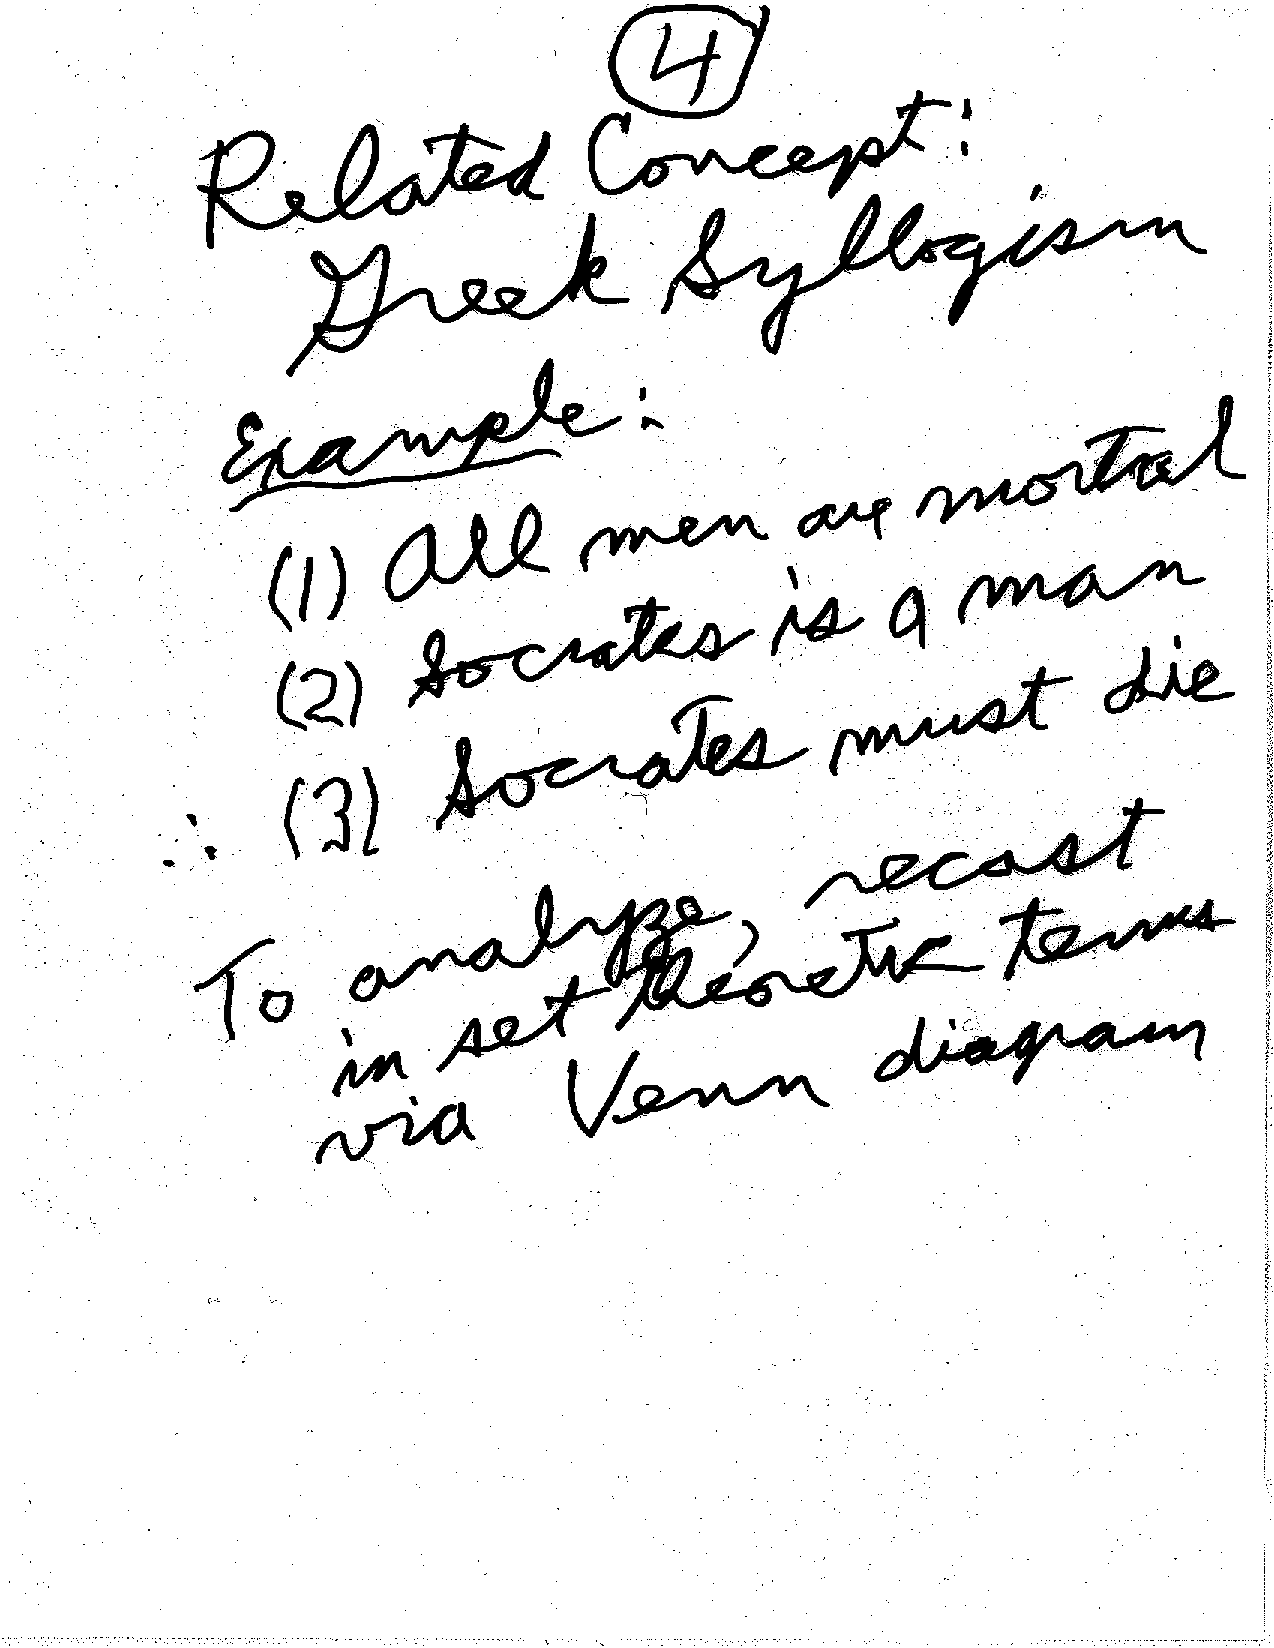
\includegraphics[scale=.5]{Pages/ST_4}

\newpage

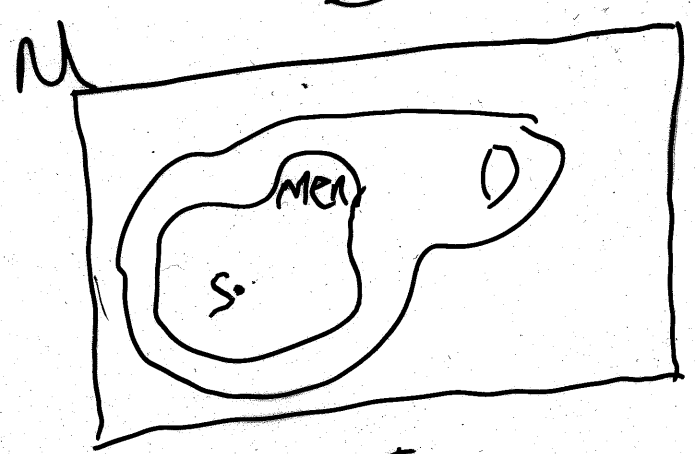
\includegraphics[scale=.2]{Pages/ST_5_im1}

$S$: Socrates\\
$M$: Set of Men\\
$D$: Things that will die\\
$\mathcal{U}$: Things on Earth

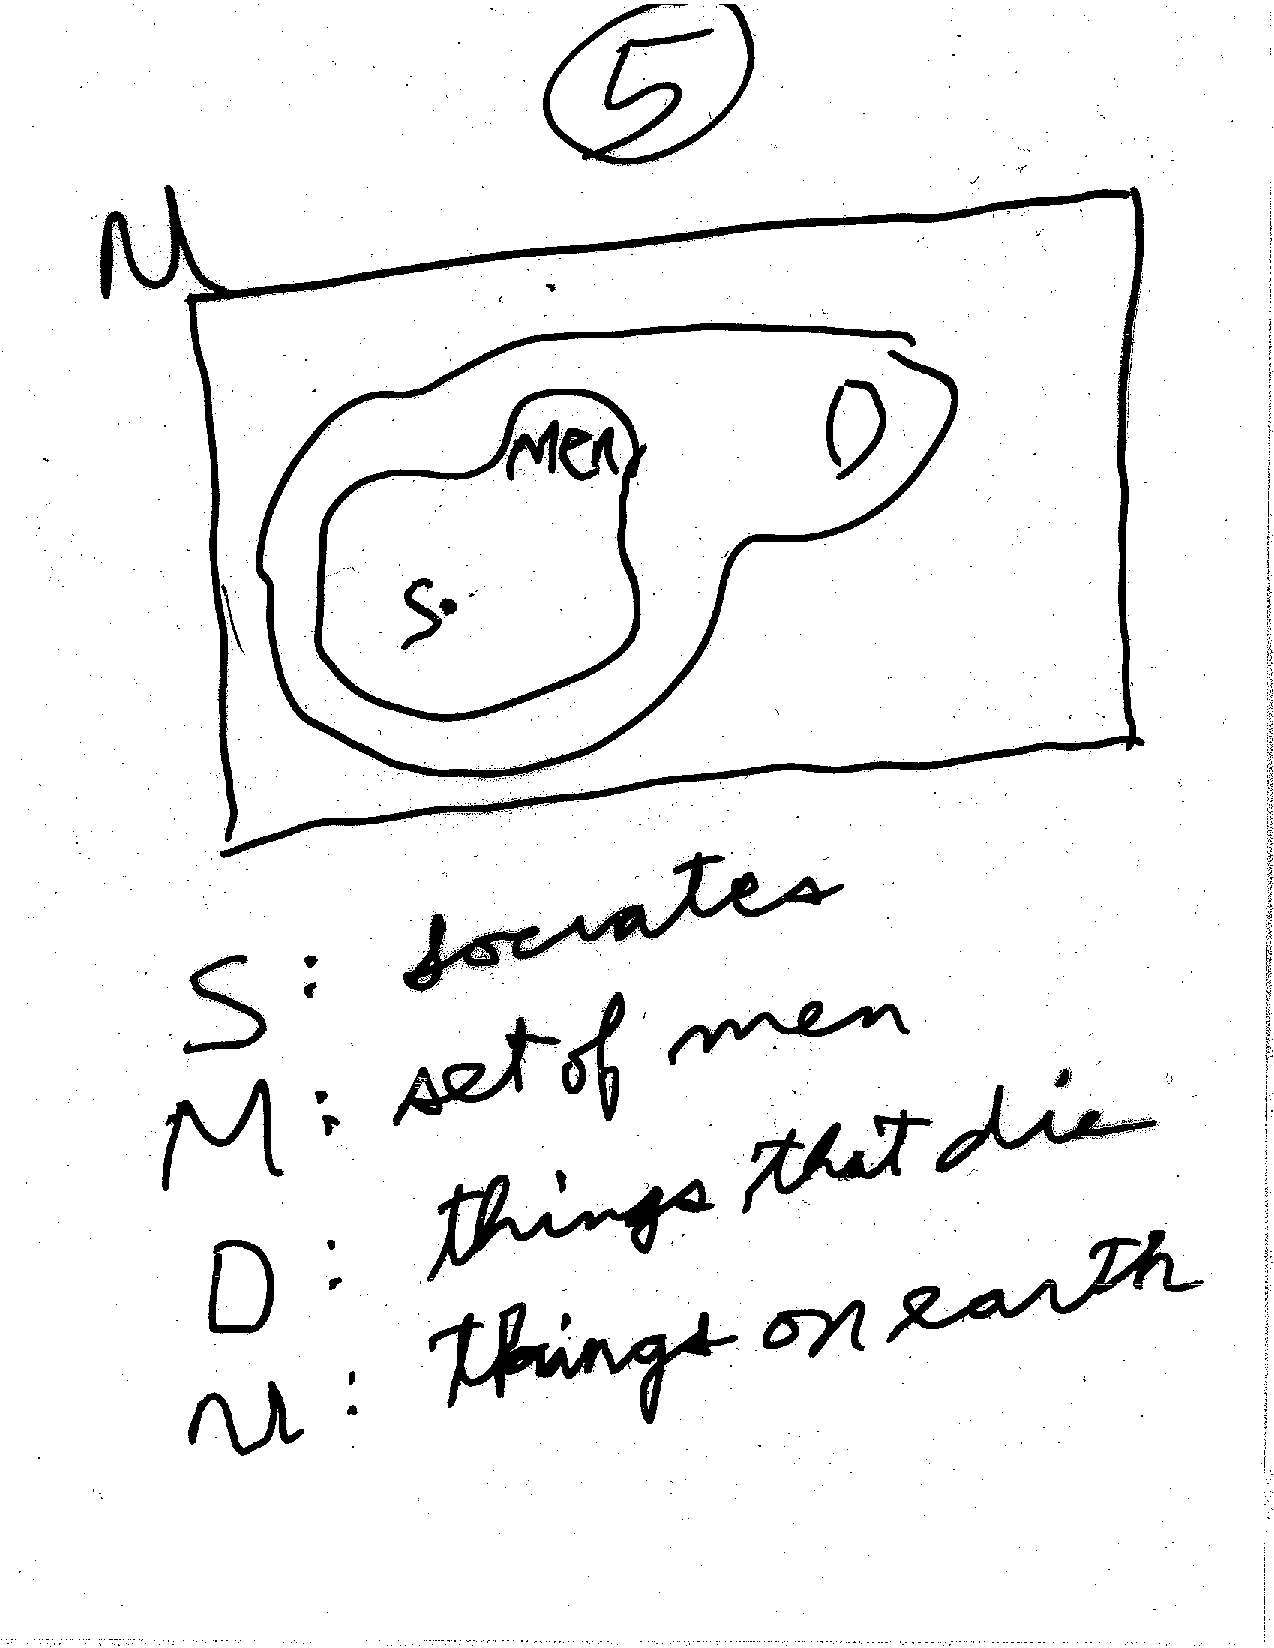
\includegraphics[scale=.5]{Pages/ST_5} 



%Zack: Pages 6,7,8,19,20

%Jack: 21, 9, 10, 11

%Koka: Pages 13, 13A, 22 ,22A, 22B


\section{Generate $\mathbb{N}$}


%Ruth: Pages L4A-L4G




\section{From $\mathbb{Z}$ to $\mathbb{R}$ via ordering}
%Jazz: ZR1-ZR5

%Kyler: ZR6 - ZR10

%Preethika: ZR11-ZR14


\section{Sequence and Limits}

%Aaron: First 2 pages and 48-50

%Hamza: 51-52B

\section{Limit and Convergence}

%Joe: 50-51

%Quinten: 52-53

%Farishta: 53A-54A

\section{Infinite Series}

%Sukhreet: IS1 - IS 7

%Matthew: IS8 - IS15

%Will: IS16 - IS23

%Rebecca: IS24 - IS32

%Maady: IS33 - IS42

\section{Metric Spaces Part 1}

%Travis: M1 - M5

%Jerome: M6- M10



\section{Metric Spaces Part 2}


%Bryant: M1-M7

%Reshma: M8-M14

%Ethan: M15-M21
\newpage

$$m15$$
\underline{Theorem} $F\subseteq M$ is closed if and only if $F^c$ is open
 
\underline{Pf} : $(\Rightarrow)$ Suppose F is closed if $F^c$ is not open $\exists  x \in F^c$ suppose that $\forall \in > o$ $\exists x_\in \neq x$ :
 $$x_\in \in D_\in (x) \bigcap F$$
Hence $x$ is a limit point of F But F contains all its limit points so $x \in F$ continued. Thus $F^c$ is open

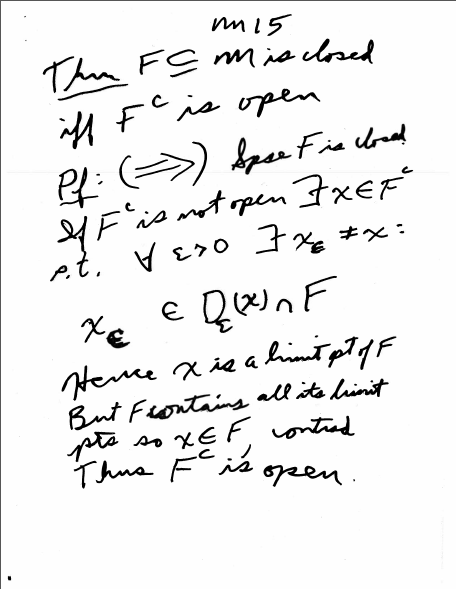
\includegraphics[scale=.75]{Pages/MS2_15}
\newpage

$$m16$$

$(\Leftarrow)$ suppose $F^c$ is open if F is not closed $\exists$ sequence of distinct points $x_n$ of F which conveys to a point $x \notin F$.
Since $x \in F^c$ and $F^c$ is open

$\exists \in > 0$ such that $D_\in$ (x) $\subset F^c$ also $\exists N : x_n \in D_e(x)$ for all $n>N$ But then $x_v \in F \bigcap F^c = \emptyset$ continued. Hence F is closed.

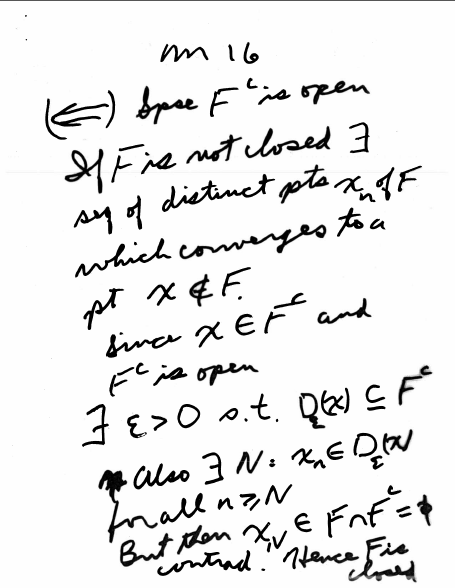
\includegraphics[scale=.75]{Pages/MS2_16}
\newpage
$$m17$$

Define let E $\leq$ m. Let E' denote the limit points of E then $\overline{E}$, the closure
 of E, is defined to be E$\bigcup$E'
\begin{itemize}
\item Fact 1 $\overline{E}$ is closed
\item Fact 2 If F is closed and E $\leq$ F then $\overline{E} \leq$ F
\end{itemize}

Corollary $\overline{E}$ = $\bigcap$ F
$/{F closed : E \leq F /}$



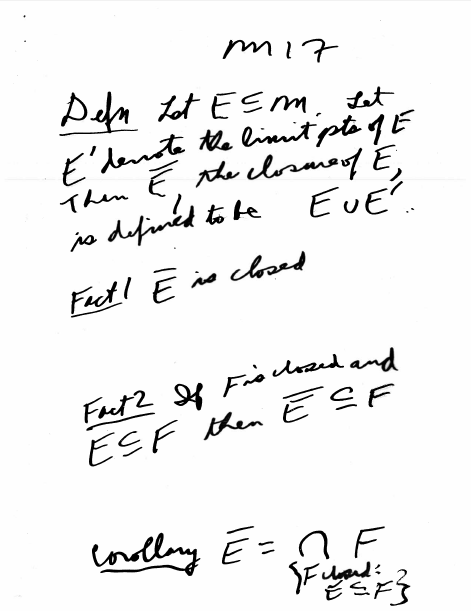
\includegraphics[scale=.75]{Pages/MS2_17}








\end{document}